\begin{boiboiboite}
	\propair
	\propgaz
	\isentropiques
\end{boiboiboite}


\subsubsection{Quelques questions de cours}

	\begin{enumerate}
		\item Pourquoi les moteurs à pistons permettent-ils d’atteindre de plus grandes températures de combustion que les turbomachines ?
		\item Quel avantage le cycle de Diesel présente-t-il sur le cycle d’Otto ?
		\item Représentez le cycle suivi par l’air dans un turboréacteur simple flux monoturbine sur un diagramme pression-volume et sur un diagramme température-entropie, de façon qualitative.
		\item Pourquoi utilise-t-on deux arbres moteur concentriques (et donc deux ensembles \{compresseur + turbine\}) dans certaines turbomachines ?
		\item Représentez le cycle suivi par l’air dans un turbomoteur à refroidisseur intermédiaire et échangeur économiseur (\cref{fig_intercooler_echangeur}) sur un diagramme température-entropie, de façon qualitative.
	\end{enumerate}

\onlyamphibook{\pagebreak}
\subsubsection{Moteur à essence}
\label{exo_cycle_moteur_essence}
\wherefrom{[partiel 2011, 6,5pts]}

	Nous nous proposons d’étudier le fonctionnement de principe du moteur à pistons/cylindres d’un avion de tourisme (\cref{fig_photos_moteur_essence}). Le moteur est dit «~à essence~» et est basé sur le cycle théorique d’Otto.
	
	\begin{figure}
		\begin{center}
			\onlyamphibook{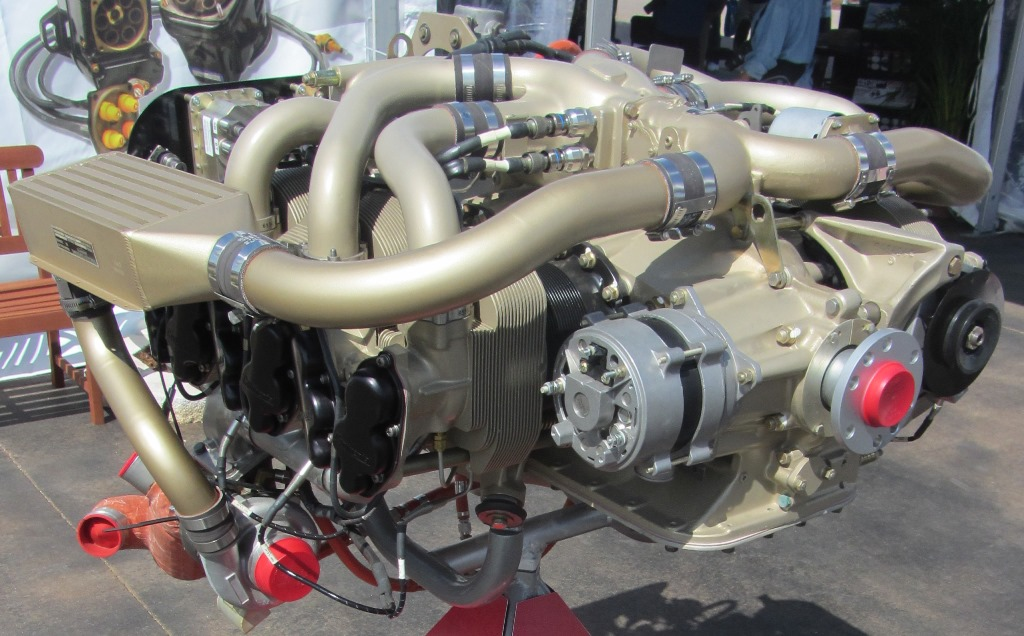
\includegraphics[width=0.8\columnwidth]{images/photo_continental_io-550.jpg}
				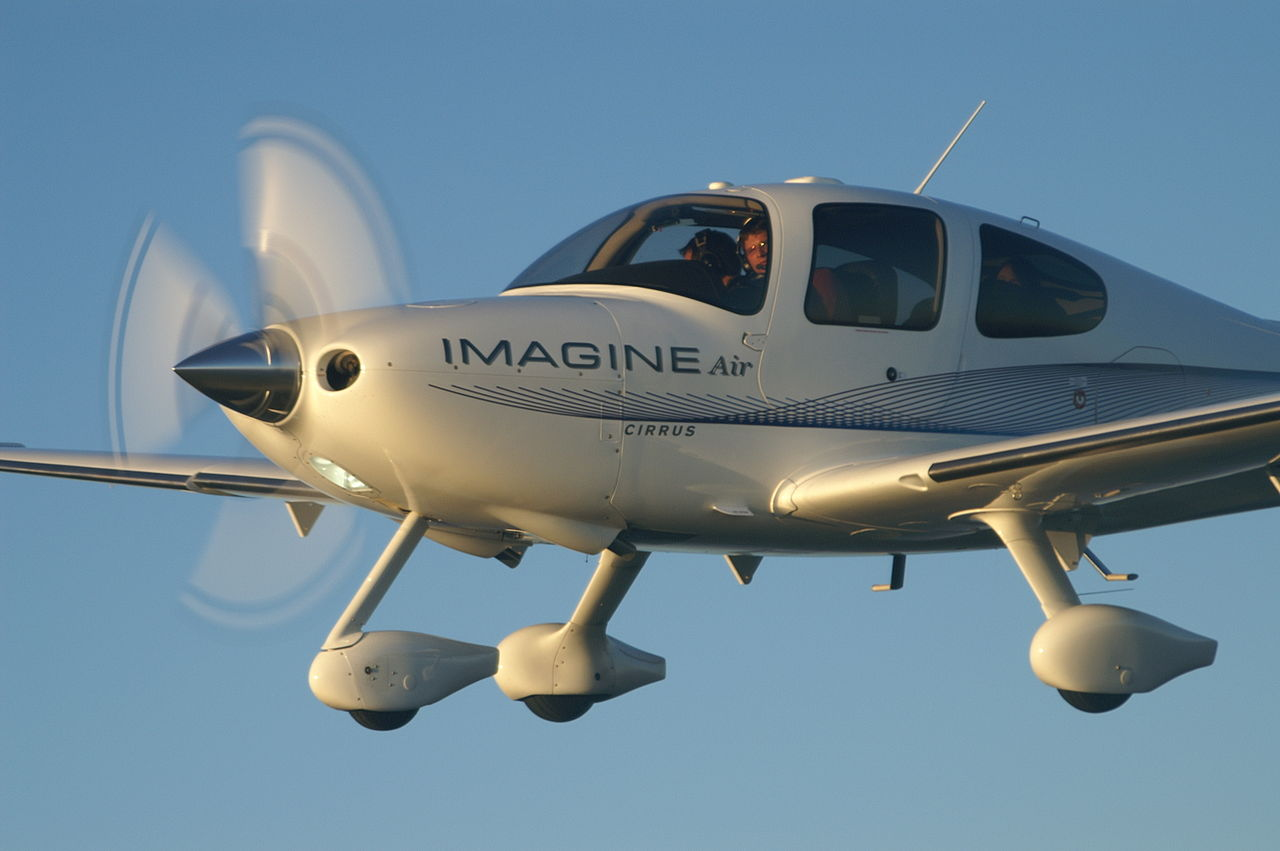
\includegraphics[width=0.8\columnwidth]{images/photo_sr22.jpg}}%handmade
			\onlyframabook{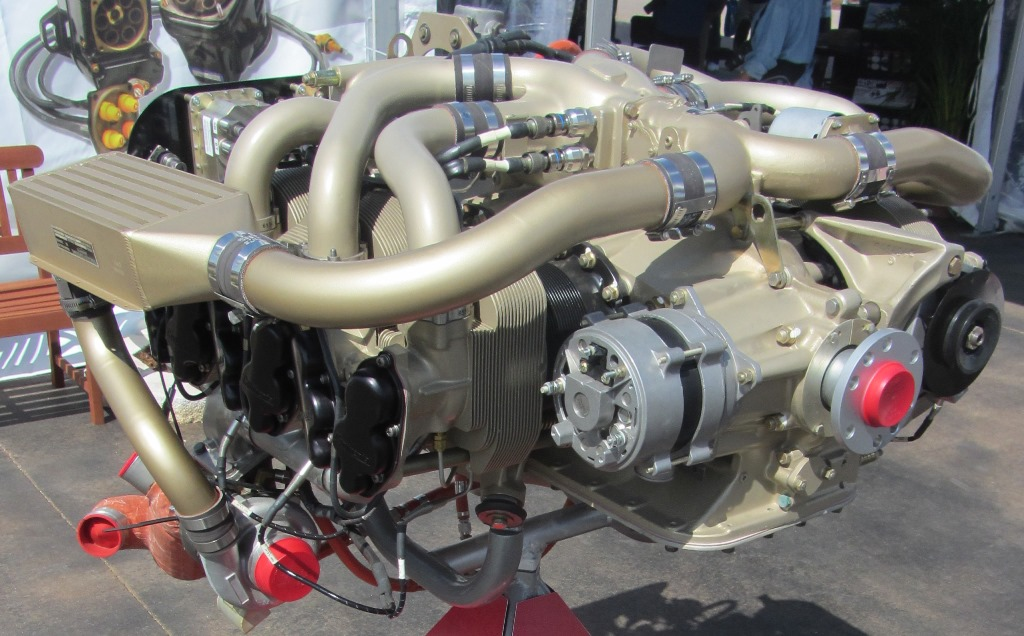
\includegraphics[width=0.9\columnwidth]{images/photo_continental_io-550.jpg}
				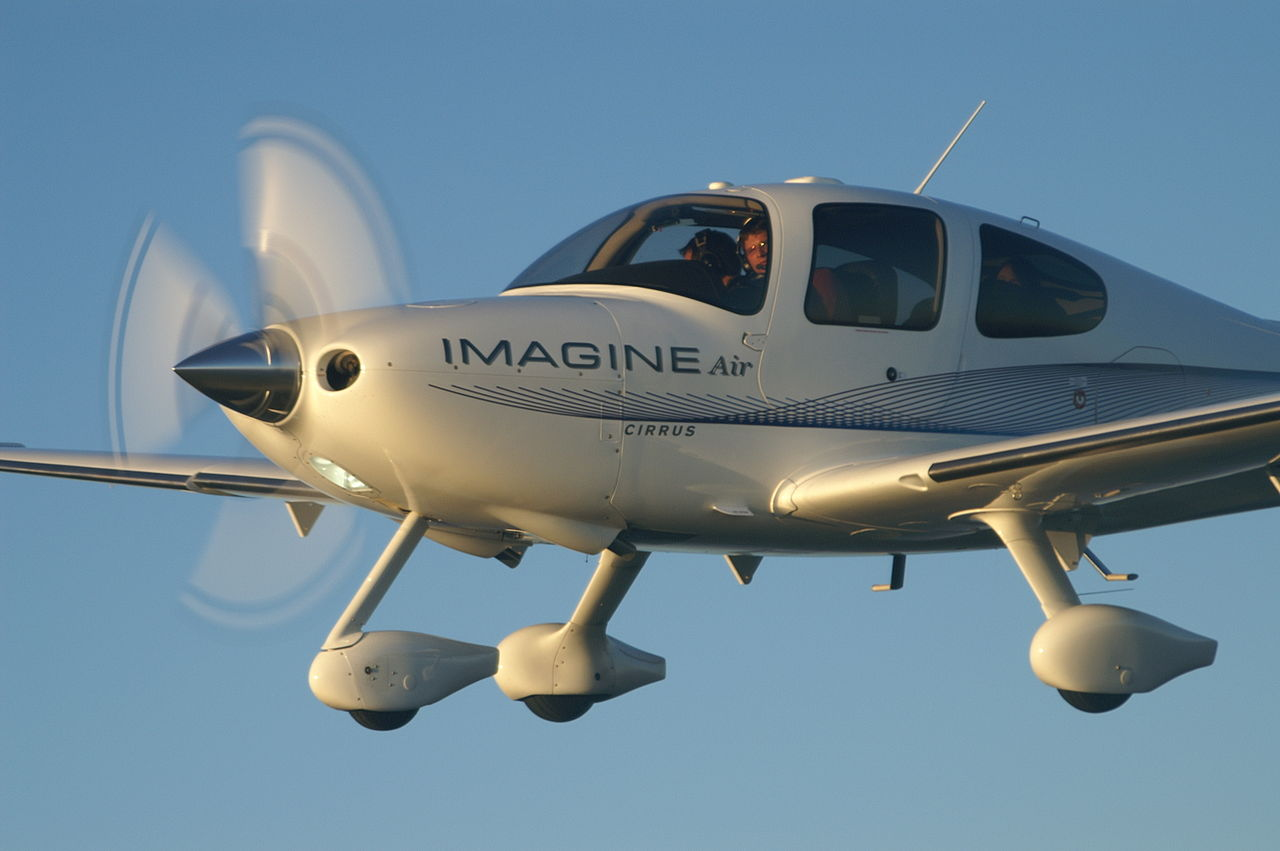
\includegraphics[width=0.9\columnwidth]{images/photo_sr22.jpg}}
		\end{center}
		\supercaption{Moteur six cylindres essence à injection \wed{Continental IO-550}{\textit{Continental} \textsc{io-550}} de~\SI{300}{ch}, en fabrication depuis 1983. Il équipe entre autres l’avion \wed{Cirrus SR22}{\textit{Cirrus} \textsc{sr22}}.\\
			Cette photo montre la version turbocompressée du moteur, dont on aperçoit l’intercooler en haut à gauche.}{\wcfile{TSIOF-550-D.jpg}{Photo moteur} \ccbysa par \wcu{FlugKerl2} ;\\ \wcfile{IAcirrus.JPG}{Photo appareil} \ccbysa par \wcu{Airman7474}.}
		\label{fig_photos_moteur_essence}
	\end{figure}
	
	\begin{itemize}
		\item Au début du cycle, l’air est à~\SI{21}{\degreeCelsius} et~\SI{1}{\bar} ;
		\item La chaleur spécifique fournie à chaque cycle pendant la croisière est de~\SI{500}{\kilo\joule\per\kilogram} ;
		\item Le taux de compression $\epsilon \equiv \frac{V_\text{max.}}{V_\text{min.}}$ est de~\num{7}.
	\end{itemize}

	Dans notre étude, nous considérons que la compression et la détente sont isentropiques et que l’apport et le rejet de chaleur se font à volume constant.

	\begin{enumerate}
		\item Tracez le cycle suivi sur un diagramme pression-volume ou température-entropie, de façon qualitative et en y représentant tous les transferts de chaleur et de travail.
		\item Quelles sont les températures de l’air au début et à la fin de la combustion ?
		\item Quelle est la quantité de chaleur rejetée lors du refroidissement ?
		\item Quel est le rendement de ce cycle moteur théorique ?
		\item En pratique, l’évolution de l’air sur le diagramme pression-volume est fort différente du cycle décrit par Otto. Proposez deux raisons expliquant cela.
		\item On constate que lorsque l’appareil gagne de l’altitude, la puissance que le moteur peut fournir baisse très significativement. Quelle modification peut-on apporter au moteur pour compenser cela ?
	\end{enumerate}


\subsubsection{Moteur Diesel}
\label{exo_cycle_moteur_diesel}
\wherefrom{[partiel 2010, 8pts]}

	Un moteur à pistons-cylindres utilisé pour propulser un navire (\cref{fig_photos_moteur_diesel}) est suralimenté par un turbocompresseur qui augmente la pression et la température de l’air d’admission à partir d’énergie extraite des gaz d’échappement (le turbocompresseur est une pièce ne nécessitant aucun apport extérieur d’énergie sous forme de travail ou de chaleur). Le moteur a ainsi les caractéristiques de fonctionnement suivantes :
	\begin{itemize}
		\item l’air admis dans les cylindres est à~\SI{115}{\degreeCelsius} et~\SI{3}{\bar} ;
		\item la chaleur spécifique fournie chaque cycle est de~\SI{1250}{\kilo\joule\per\kilogram} ;
		\item le taux de compression $\epsilon \equiv \frac{V_\text{max.}}{V_\text{min.}}$ est de~\num{17}.
	\end{itemize}
	
	\begin{figure}
		\begin{center}
			\onlyamphibook{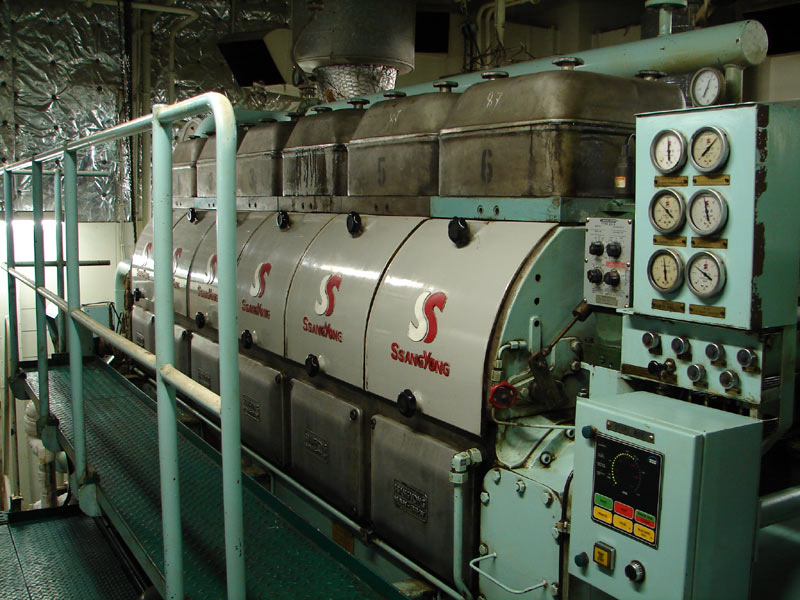
\includegraphics[width=0.9\columnwidth]{images/photo_diesel_generateur.jpg}
				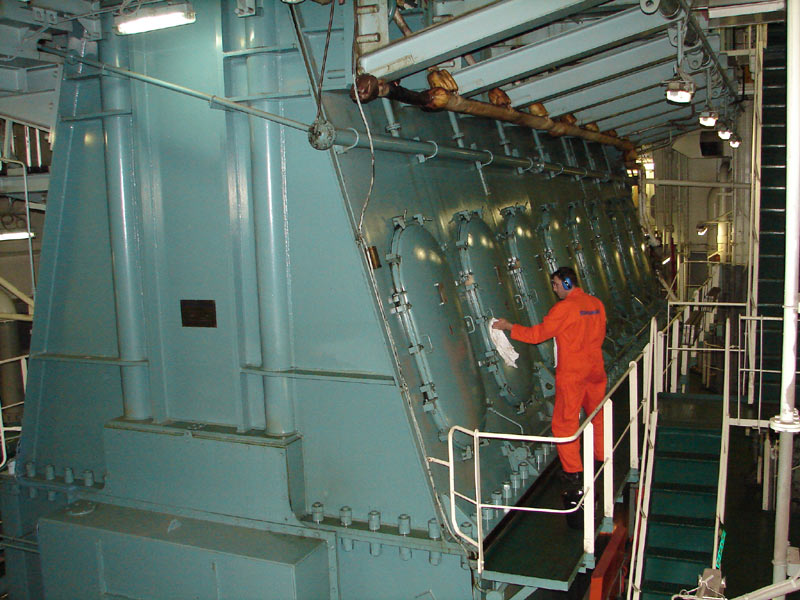
\includegraphics[width=0.9\columnwidth]{images/photo_diesel_propulsion.jpg}}
			\onlyframabook{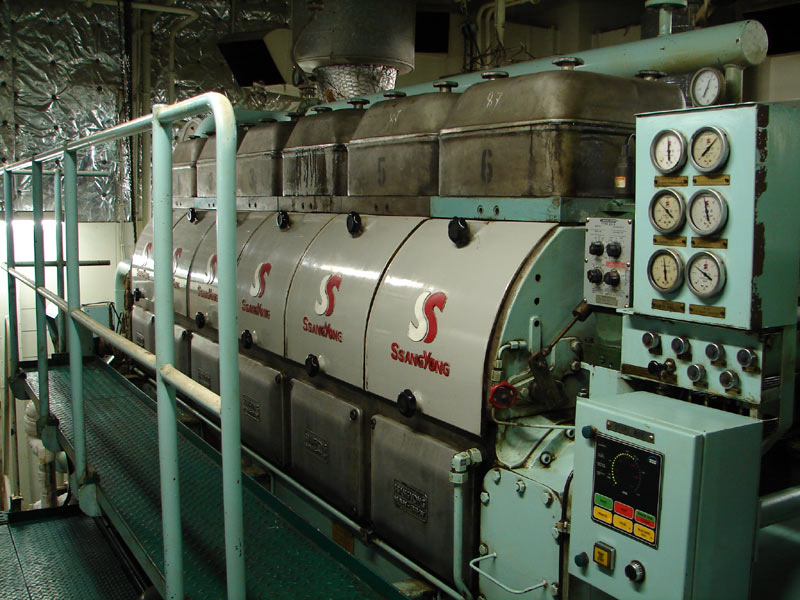
\includegraphics[width=0.49\textwidth]{images/photo_diesel_generateur.jpg}
				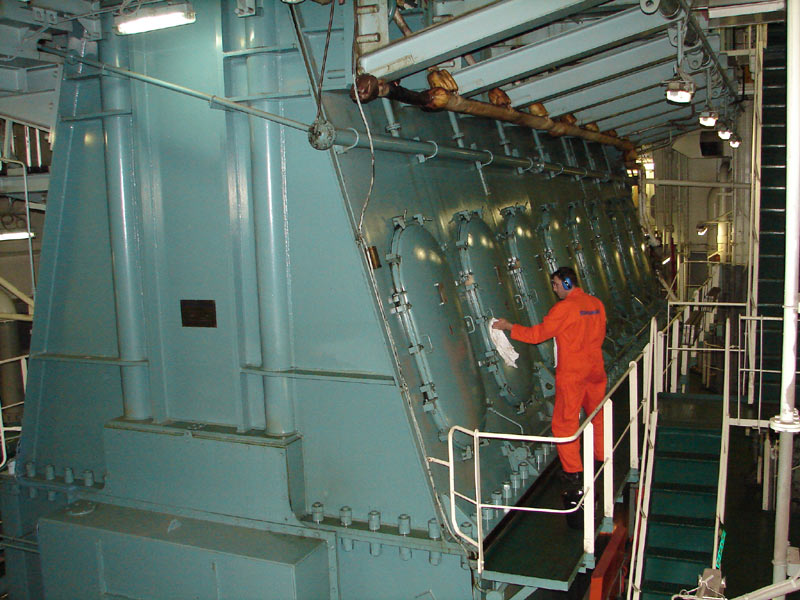
\includegraphics[width=0.49\textwidth]{images/photo_diesel_propulsion.jpg}}
		\end{center}
		\supercaption{Moteurs Diesel six cylindres de~\SI{1100}{\kilo\watt} électrogène (gauche) et sept cylindres de~\SI{25}{\mega\watt} propulsif (droite) d’un pétrolier de~\SI{290 000}{\tonne}.}{\wcfile{Diesel generator on an oil tanker.jpg}{Photo 1} et \wcfile{Main engine of a VLCC tanker 3.jpg}{2} \ccbysa par Hervé Cozanet}
		\label{fig_photos_moteur_diesel}
	\end{figure}

	Nous considérons le cas de fonctionnement optimal, c’est à dire le suivi du cycle de Diesel, selon les caractéristiques suivantes :
	\begin{itemize}
		\item compression et détente isentropiques ;
		\item combustion à pression constante ;
		\item rejet de chaleur à volume constant.
	\end{itemize}
	
	\begin{enumerate}
		\item Tracez le cycle thermodynamique suivi sur un diagramme pression-volume ou température-entropie, de façon qualitative et en y indiquant tous les transferts de chaleur et de travail.
		\item Quelle est la température de l’air à la fin de la compression ?
		\item Quelle est la température des gaz à la fin de la combustion ?
		\item Quelle est la pression maximale atteinte dans le moteur ?
		\item Quelle est la température à la fin de la détente ?
		\item Quel est le rendement du moteur ?
		\item Il est aisé de montrer qu’à taux de compression égal, un cycle Diesel est moins efficace qu’un cycle dit «~à essence~» (cycle d’Otto). Pourquoi est-il alors utilisé ?
	\end{enumerate}


\subsubsection{Turbopropulseur}
\label{exo_cycle_turbopropulseur}
\wherefrom{[calqué sur partiel 2010, 7pts]}
	
	Un avion de ligne régional est motorisé par deux turbopropulseurs (\cref{fig_turboprop_photos}). Dans chacun d’entre eux, une turbine unique alimente un compresseur axial, ainsi que l’hélice par l’intermédiaire d’un réducteur (\cref{fig_turboprop_circuit}).
	
	\begin{figure}
		\begin{center}
			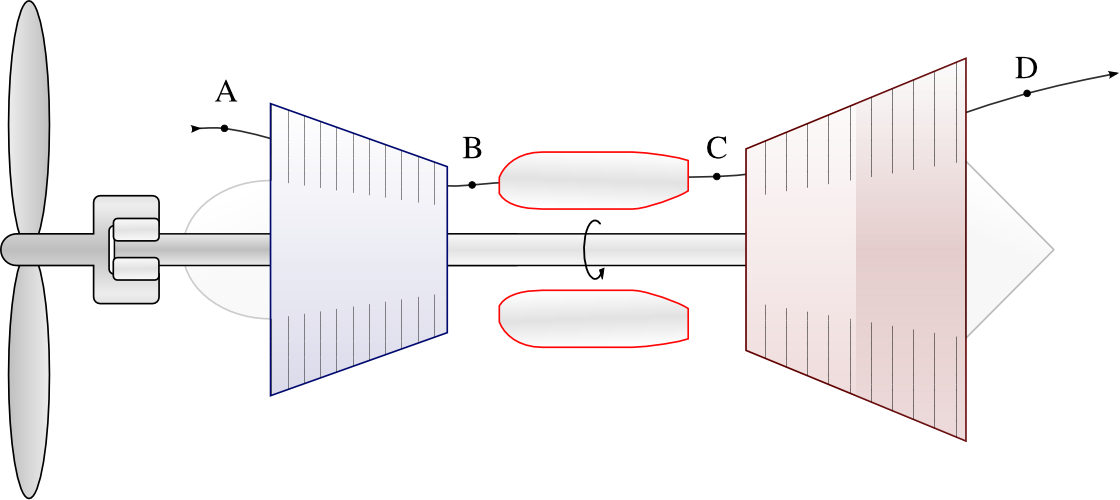
\includegraphics[width=11cm]{images/circuit_turboprop.png}
		\end{center}
		\supercaption{Agencement interne de principe d’un turbopropulseur.}{schéma \ccbysa \olivier}
		\label{fig_turboprop_circuit}
	\end{figure}
	
	Pendant la croisière, le débit d’air au sein du moteur est de~\SI{4,9}{\kilogram\per\second}, et le circuit est le suivant :
	\begin{itemize}
		\item L’air à pression et température ambiantes (\SI{0,55}{\bar} \&~\SI{-5}{\degreeCelsius}) est admis dans le compresseur ;
		\item Le compresseur porte l’air à pression de~\SI{7,6}{\bar} avec une efficacité isentropique de~\SI{80}{\percent} ;
		\item L’air est ensuite chauffé dans la chambre de combustion jusqu’à~\SI{1315}{\degreeCelsius} ;
		\item Les gaz de combustion sont ensuite détendus dans la turbine et rejetés dans l’atmosphère ; la turbine a une efficacité isentropique de~\SI{80}{\percent}.
	\end{itemize}
	
	 La turbine alimente le compresseur (par l’intermédiaire d’un axe aux frottements négligeables) et l’hélice (par l’intermédiaire d’une boîte de transmission d’efficacité~\SI{83}{\percent}).
	
	Nous souhaitons quantifier la puissance effectivement reçue par l’hélice au cours du vol.
	
	\begin{enumerate}
		\item Tracez le cycle suivi par l’air sur un diagramme température-entropie, de façon qualitative.
		\item Quelle est la température de l’air à la sortie du compresseur ?
		\item Quelle est la température des gaz à la sortie de la turbine ?
		\item Quelle est la puissance fournie à l’hélice ?
	\end{enumerate}

	Afin de procéder au dégivrage des ailes, on effectue un petit prélèvement de gaz au sein du compresseur. Le débit du prélèvement est de~\SI{0,1}{\kilogram\per\second}, et la température de l’air est de~\SI{200}{\degreeCelsius}.
	
	\begin{enumerate}
		\shift{4}
		\item Proposez et quantifiez une modification à porter au fonctionnement du moteur pour qu’il puisse fournir la même puissance à l’hélice.
	\end{enumerate}
	
	\onlyamphibook{\begin{figure}[h!]}
	\onlyframabook{\begin{figure}[htc]}%handmade
		\begin{center}
			\onlyamphibook{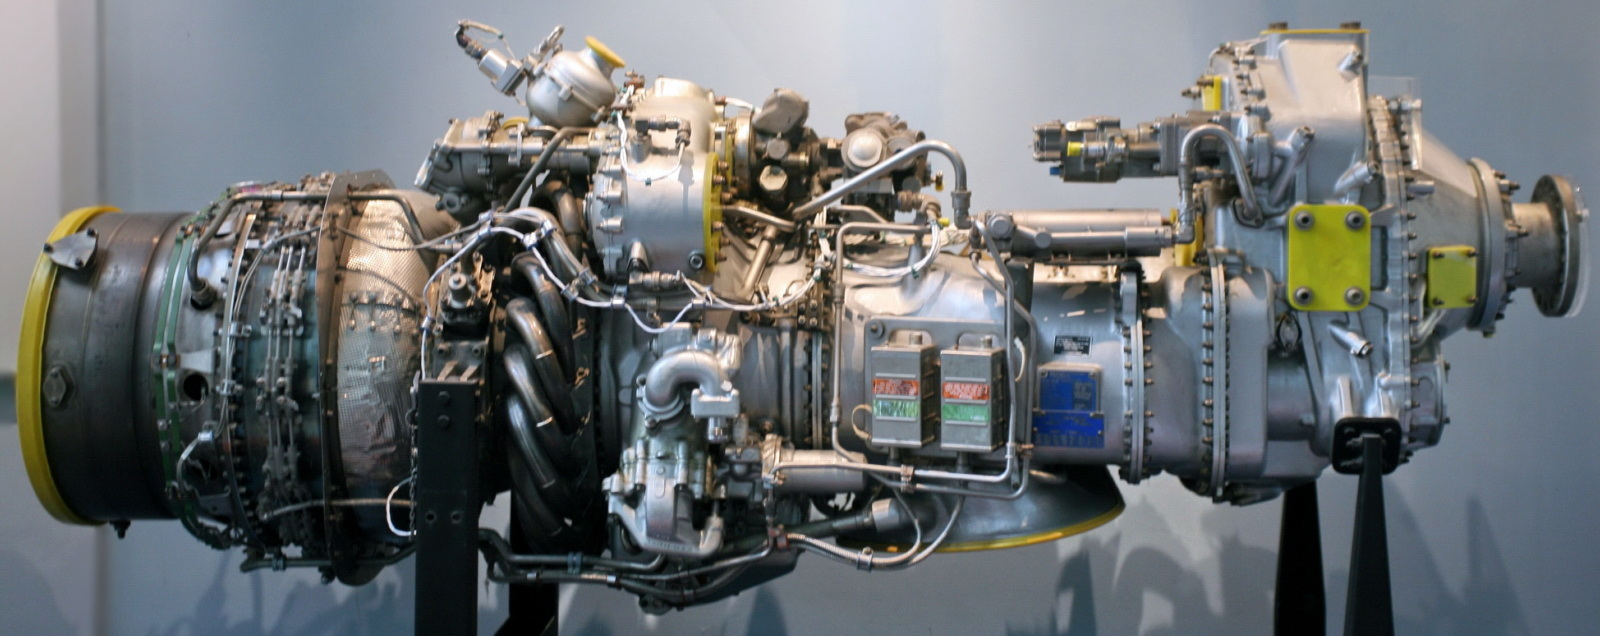
\includegraphics[width=0.9\columnwidth]{images/photo_pwc_pw123.jpg}
				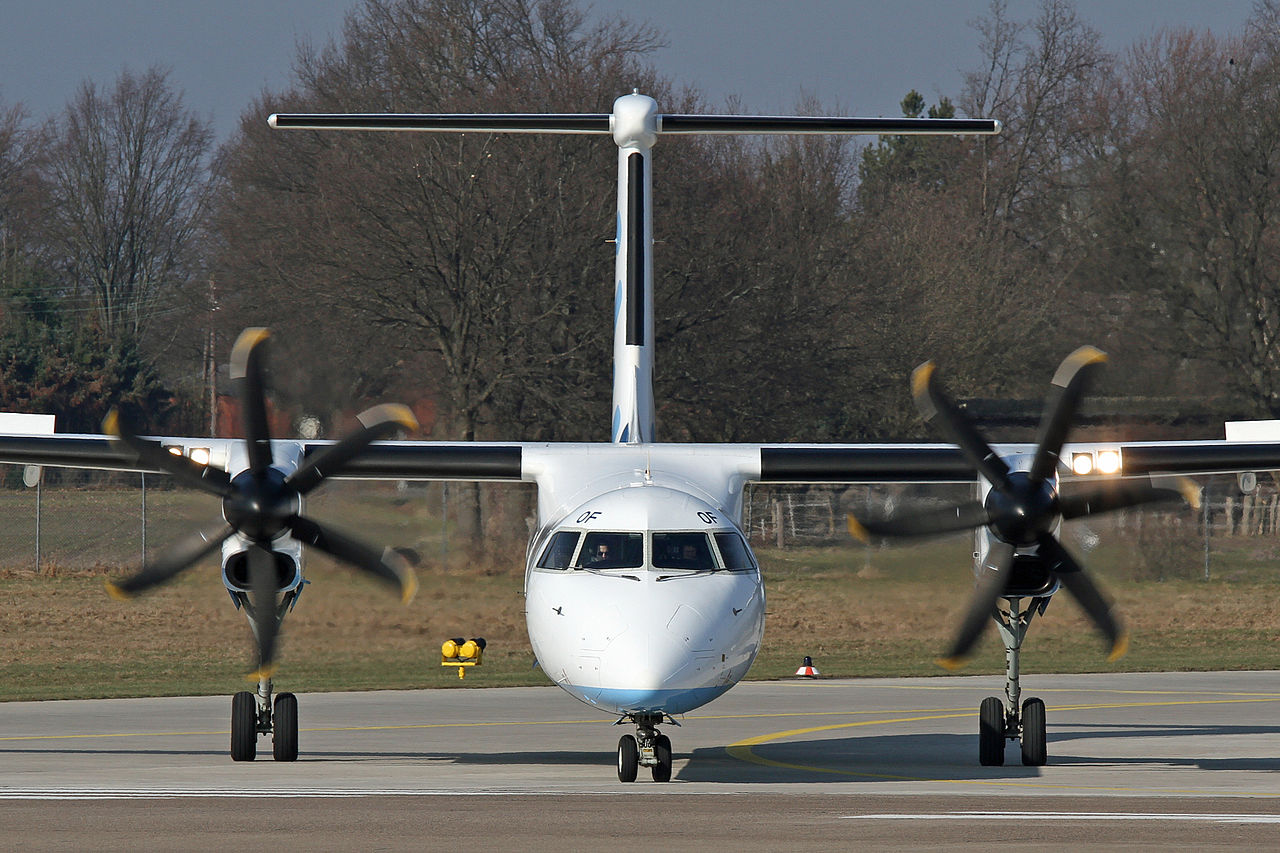
\includegraphics[width=0.9\columnwidth]{images/photo_dash8.jpg}}
			\onlyframabook{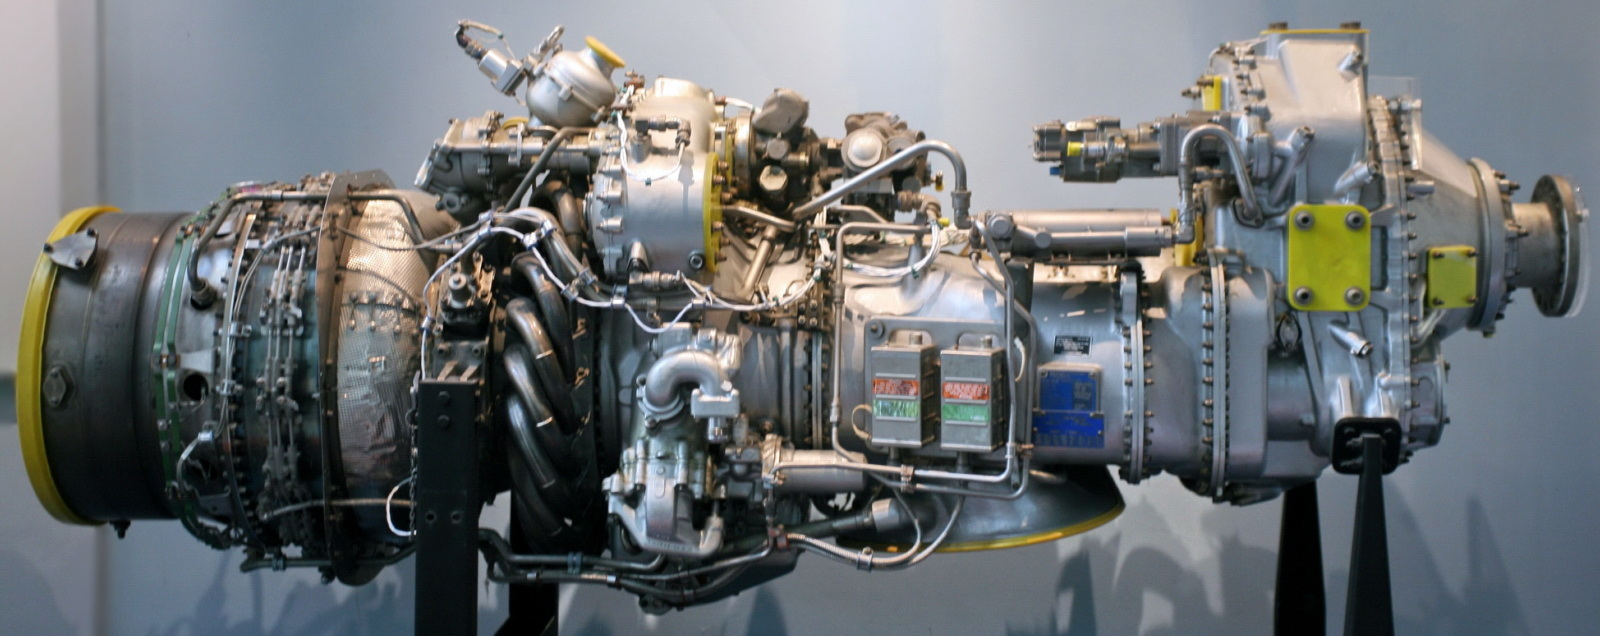
\includegraphics[width=\columnwidth]{images/photo_pwc_pw123.jpg}
				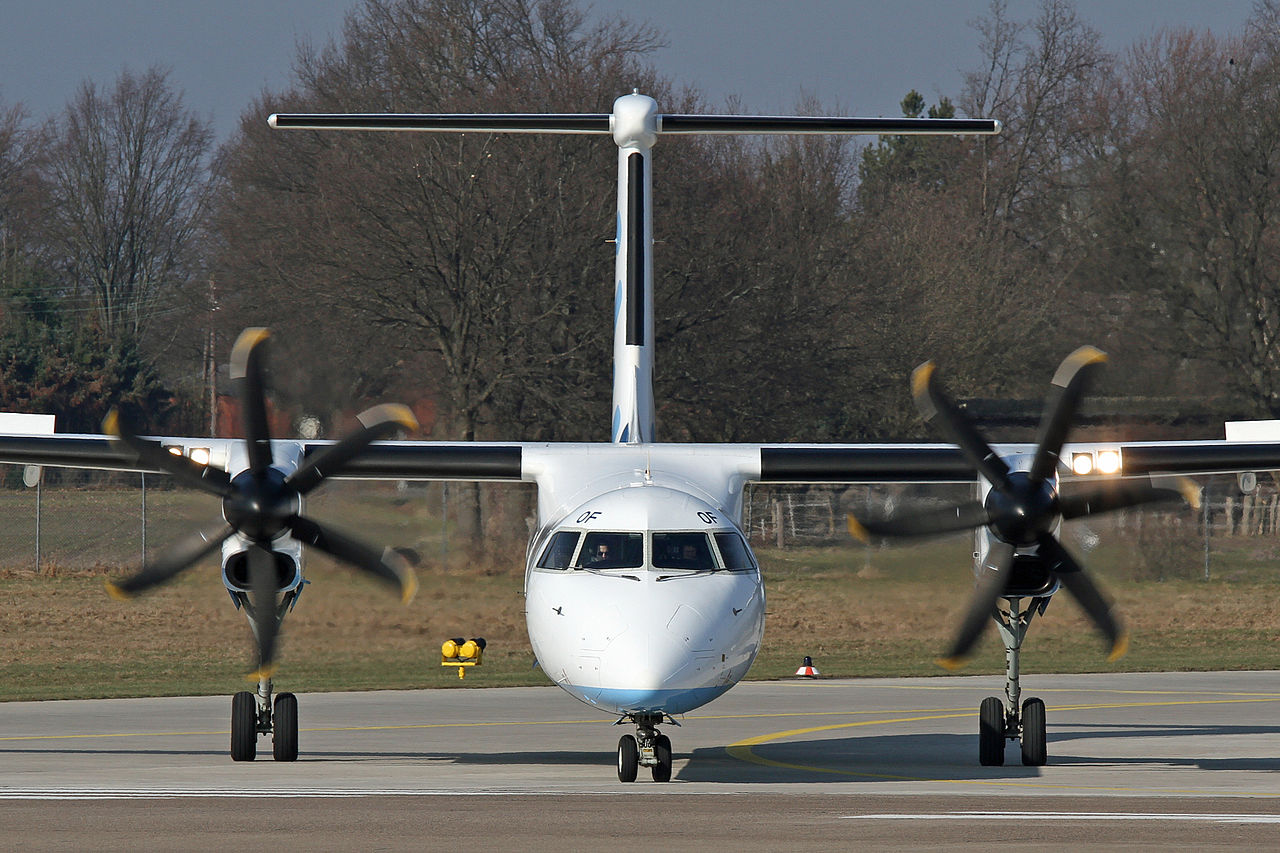
\includegraphics[width=\columnwidth]{images/photo_dash8.jpg}}
		\end{center}
		\supercaption{Un turbopropulseur \textit{Pratt \& Whitney Canada} \textsc{pwc123} équipant un \textit{Bombardier} Dash~8. Le \textsc{pwc123} est configuré avec trois ensembles tournants concentriques, dont l’arbre moteur alimenté par un turbine libre, mais son agencement de principe reste similaire à celui décrit en \cref{fig_turboprop_circuit}.}%
{\wcfile{Pratt & Whitney Canada PW123 retouched.jpg}{Photo moteur} dérivée d’\wcfile{Pratt & Whitney Canada PW123.jpg}{une photo} \ccby par \href{http://www.flickr.com/people/28567825@N03}{l’utilisateur$\cdot$rice flickr cliff1066} ; \wcfile{Dash 8 front view.jpg}{Photo avion} \ccbysa par \href{http://www.flickr.com/people/24056116@N07}{l’utilisateur$\cdot$rice Flickr Björn}}
		\label{fig_turboprop_photos}
	\end{figure}
		
\onlyamphibook{~\par\vspace{10cm}}%handemade carrément pourri
\subsubsection{Modification de turboréacteur}
\label{exo_cycle_turboreacteur}

	Un turboréacteur monoflux fonctionne avec un seul axe moteur (compresseur unique et turbine unique). Ses caractéristiques de fonctionnement sont les suivantes :
		\begin{itemize}
			\TabPositions{0.55\columnwidth} %handmade, pour faire tenir les données
			\item Débit d’air :							\tab \SI{4}{\kilogram\per\second}
			\item Conditions atmosphériques : 		\tab \SI{283}{\kelvin} \& \SI{0,95}{\bar}
			\item Rapport de pression $\frac{p_\text{max.}}{p_\text{min.}}$ : 				\tab \num{25}
			\item Température maximale : 													\tab \SI{1300}{\kelvin}
			\item Efficacité isentropique du compresseur et de la turbine : 	\tab \SI{85}{\percent}
		\end{itemize}
	
	On cherche à quantifier ses performances avant modification.
		\begin{enumerate}
			\item Représentez les composants du turboréacteur et le cycle thermodynamique suivi par l’air sur un diagramme température-entropie ou pression-volume.
			\item Quelle est la pression disponible à la sortie de la turbine ?
			\item Quelle serait la vitesse atteinte par les gaz en sortie de tuyère si la détente y était isentropique ?
		\end{enumerate}

	\onlyamphibook{\begin{figure}}
	\onlyframabook{\begin{figure}[htc]}%handmade
		\begin{center}
			\onlyamphibook{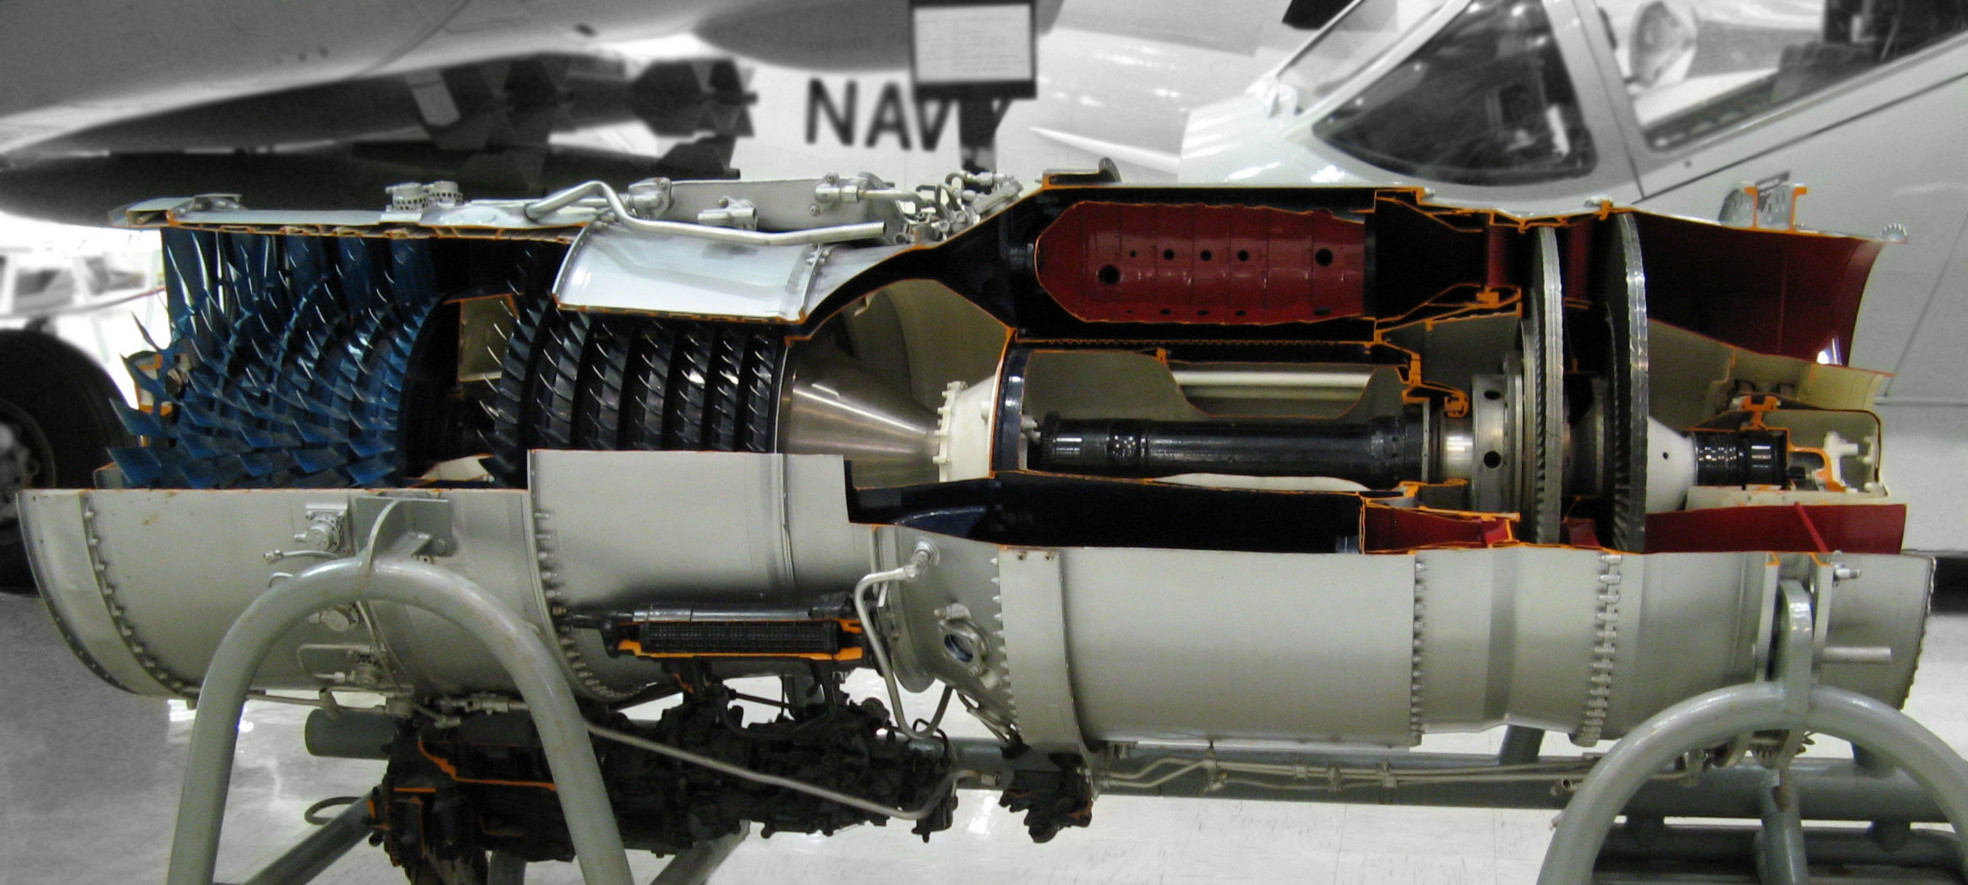
\includegraphics[width=\columnwidth]{images/photo_pw_j52_1.jpg}}
			\onlyframabook{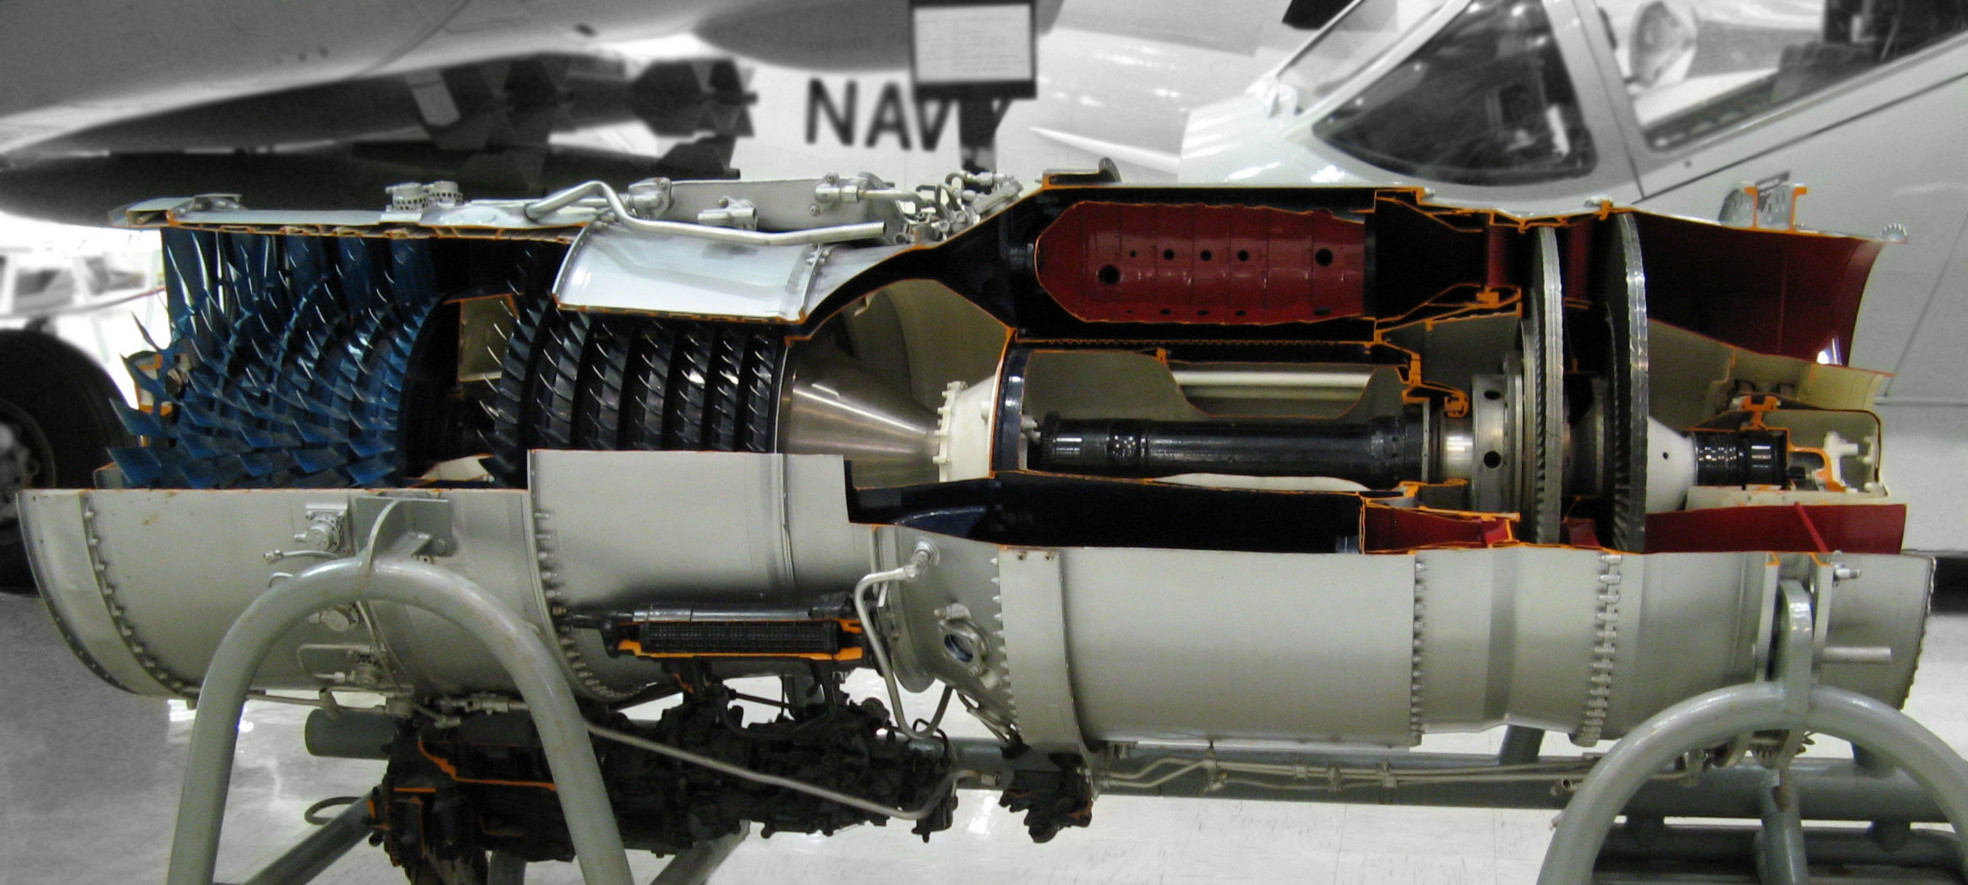
\includegraphics[width=\columnwidth]{images/photo_pw_j52_1.jpg}
				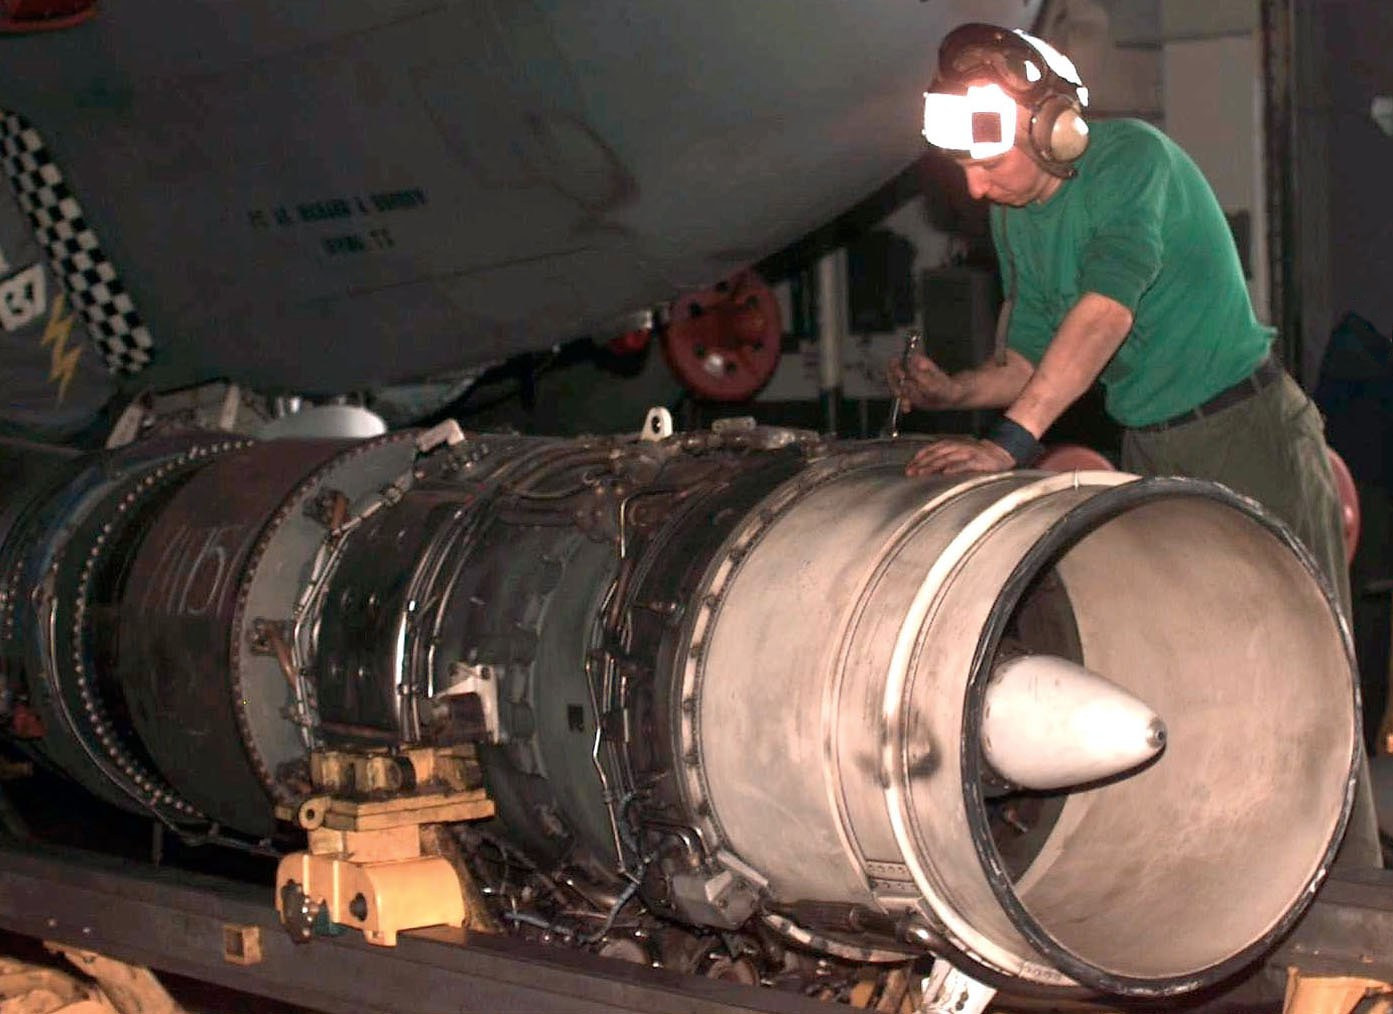
\includegraphics[width=\columnwidth]{images/photo_pw_j52_2.jpg}}
		\end{center}
		\supercaption{Un turboréacteur à simple flux et deux arbres \wed{Pratt & Whitney J52}{\textit{Pratt \& Whitney} \textsc{j52}} (ou \textsc{jt8a}), construit en \num{4500} exemplaires. Il équipe encore le \wed{Northrop Grumman EA-6B Prowler}{\textsc{ea-6b} \textit{Prowler}}.}%
		{Photo 1 dérivée d’\wcfile{Pratt & Whitney J52.jpg}{une photo} \ccby par \href{http://www.flickr.com/people/37467370@N08}{Greg Goebel} ; Photo 2 dérivée d’\wcfile{J52 engine maintenance USS America (CV-66) 1993.JPEG}{une photo} \pd par Sgt. G. Robinson, U.S.~Navy}
		\label{fig_exo_turbojet_twin_spool}
	\end{figure}

		\onlyframabook{\pagebreak}
		L’équipe d’ingénieurs en charge de la conception des composants propose de modifier le moteur, en utilisant deux axes plutôt qu’un seul (\cref{fig_exo_turbojet_twin_spool}). L’ensemble tournant le plus au centre du moteur pouvant évoluer à plus grande vitesse, l’efficacité isentropique des composants est augmentée :
			\begin{itemize}
				\item Efficacité isentropique du compresseur et de la turbine basse pression (axe \textsc{bp}) : \SI{85}{\percent}\\
					(rapport des pressions : \num{2})
				\item Efficacité isentropique du compresseur et de la turbine haute pression (axe \textsc{hp}) : \SI{90}{\percent}\\
					(rapport des pressions : \num{12,5})
			\end{itemize}
	
	
			
		Toutes les autres caractéristiques de fonctionnement du moteur restent inchangées.
		
		\begin{enumerate}
		\shift{3}
			\item Quelle est la nouvelle pression disponible à la sortie de la turbine ?
			\item Quelle est la nouvelle vitesse théorique d’éjection des gaz ?
		\end{enumerate}

\onlyamphibook{\pagebreak}
\subsubsection{Turbomoteur à refroidissement intermédiaire}
\label{exo_cf6_generateur_intercooling}

	Vous êtes chargé/e par une petite entreprise de développer un moteur qui sera destiné à générer de l’électricité dans une usine. Il est décidé de baser le moteur sur un turboréacteur à soufflante issu d’un avion de ligne retiré du service : il s’agit d’un vénérable \textit{General Electric} \textsc{cf6} (figures~\ref{fig_cf6_1} et~\ref{fig_cf6_2}).
	
	\begin{figure}
		\begin{center}
		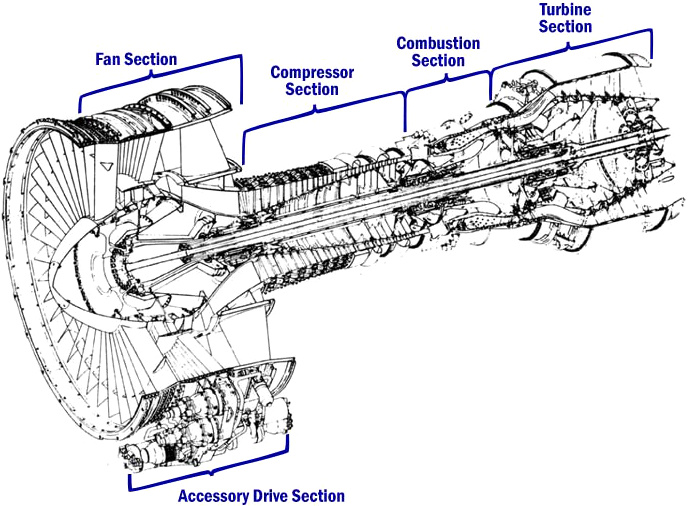
\includegraphics[width=10cm]{images/cf6_cutaway.jpg}
		\end{center}
		\supercaption{Schéma de coupe d’un \wed{General Electric CF6}{\textit{General Electric} \textsc{cf6-6}}. Le moteur a propulsé toutes les grandes familles d’appareils long-courrier des années~70 et~80.}{\wcfile{CF6-6 engine cutaway.jpg}{schéma} \pd U.S. FAA}
		\label{fig_cf6_1}
	\end{figure}
	
	\begin{figure}
		\begin{center}
		\onlyamphibook{\vspace{-0.5cm}}
		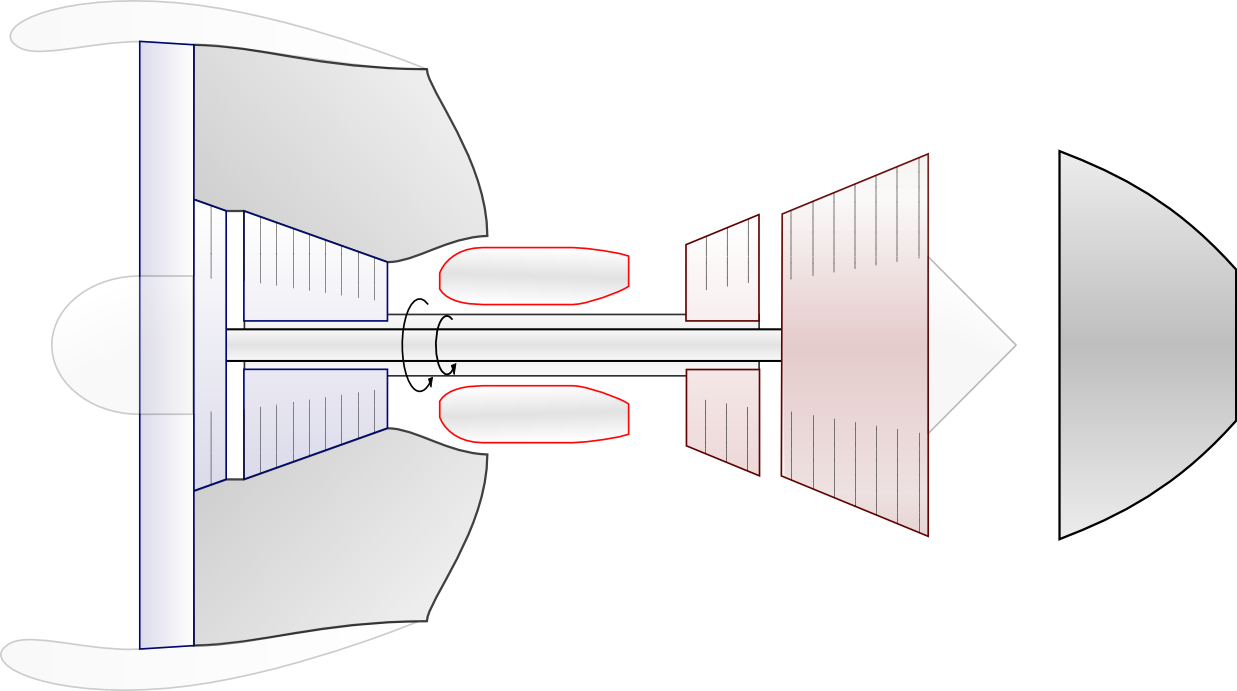
\includegraphics[width=10cm]{images/circuit_turbofan_twin_spool.png}
		\end{center}
		\supercaption{Schéma de principe de l’agencement du \textit{General Electric} \textsc{cf6}.}{schéma \ccbysa \olivier}
		\label{fig_cf6_2}
	\end{figure}
	
	Le turboréacteur possède deux axes concentriques :
		
	\begin{itemize}
		\item L’axe basse pression relie la soufflante, une section de compresseur appelée \textit{booster} et la turbine basse pression ;
		\item L’axe haute pression relie le reste du compresseur et la turbine haute pression.
	\end{itemize}	

	Le turboréacteur a les propriétés suivantes :
		
	\begin{description}
		\TabPositions{0.7\columnwidth} %handmade, pour faire tenir les données
		\item Rapport maximal des pressions : 						\tab \num{29,3}
		\item Rapport des pressions du booster : 					\tab \num{1,2}
		\item Rapport des pressions de la soufflante : 			\tab \num{1,2}
		\item Température maximale : 									\tab \SI{1300}{\degreeCelsius}
		\item Efficacité isentropique des compresseurs : 		\tab \SI{85}{\percent}
		\item Efficacité isentropique des turbines : 			\tab \SI{85}{\percent}
		\item Pression de rejet des gaz dans l’atmosphère : 	\tab \SI{1,1}{\bar}
	\end{description}

	Pour transformer le turboréacteur en turbomoteur, vous faites retirer la nacelle et la soufflante, et vous faites connecter mécaniquement l’axe basse pression à la génératrice (\cref{fig_turbomoteurs_exercice}). Le turbomoteur est mis en route aux conditions atmosphériques de~\SI{1}{\bar} et~\SI{18}{\degreeCelsius}. À plein régime, il utilise un débit d’air de~\SI{80}{\kilogram\per\second}.
	
	\begin{enumerate}
		\item Représentez le cycle thermodynamique suivi par l’air sur un diagramme pression-volume, de façon qualitative.
		\item Quelle est la puissance mécanique développée par la machine ?
		\item Quelle est sa marge de travail ?
		\item Quelle est son efficacité ?
	\end{enumerate}
	
	\onlyframabook{\pagebreak}%handmade
	L’entreprise cliente réceptionne votre moteur mais souhaite augmenter la puissance qu’il développe. Le moteur fonctionnant déjà à pleine capacité, vous n’êtes en mesure d’augmenter ni le débit d’air, ni la température de combustion.
	
	Pour pouvoir augmenter la puissance, vous installez un système d’intercooling (figure~\ref{fig_turbomoteurs_exercice}). La compression de l’air est interrompue à pression de~\SI{7}{\bar} ; l’air est conduit dans un grand échangeur de chaleur où il est refroidi à pression constante. Lorsque sa température est redescendue à~\SI{40}{\celsius}, on reprend sa compression dans le compresseur, qui n’a pas été modifié.
	
	\begin{enumerate}
	\shift{4}	
		\item Représentez qualitativement le nouveau cycle thermodynamique sur le diagramme pression-volume plus haut.
		\item De combien augmente la puissance mécanique développée par la machine ?
		\item Quelle est la nouvelle marge de travail ?
		\item Quelle est la nouvelle efficacité ?
	\end{enumerate}
	
	\onlyframabook{\pagebreak}%handmade
	\begin{figure}[htc!]%handmade
		\begin{center}
		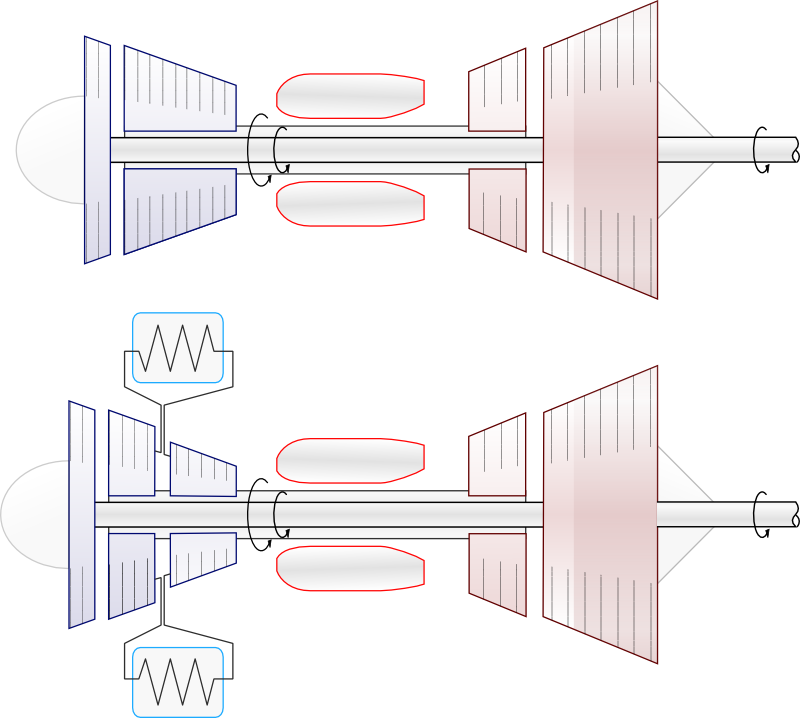
\includegraphics[width=12cm]{images/circuit_turboshaft_exercice.png}
		\end{center}
		\supercaption{	En haut : schéma de principe d’un turbomoteur basé sur le \textsc{cf6} dont on a supprimé la soufflante.\\
							En bas : le même turbomoteur modifié par l’ajout d’un système de refroidissement intermédiaire (intercooler).}{schémas \ccbysa \olivier}
		\label{fig_turbomoteurs_exercice}
	\end{figure}

\exercisesolutionpage
\titreresultats
	
	\begin{description}
		\item [\ref{exo_cycle_moteur_essence}]
			\tab 1) Voir \cref{fig_cycle_otto} ;
	 		\tab 2) $T_\B = T_\A \left(\frac{v_\A}{v_\B}\right)^{\gamma_\text{air} - 1} = \SI{640,6}{\kelvin} = \SI{367,5}{\degreeCelsius}$ (\ref{eq_isentropique_horrible1}) et $T_\C = \frac{q_\text{combustion}}{c_{v \text{(gaz)}}} + \frac{c_{v \text{(air)}}}{c_{v \text{(gaz)}}} T_\B = \SI{1166,3}{\kelvin} = \SI{893,3}{\degreeCelsius}$ ;
	 		\tab 3) $T_\D = \SI{610,16}{\kelvin} = \SI{337}{\degreeCelsius}$ (\ref{eq_isentropique_horrible1}) ainsi $q_\fromdtoa = c_{v \text{(gaz)}} (T_\D - T_\A) = \SI{-260,1}{\kilo\joule\per\kilogram}$ ;
	 		\tab 4) $\eta_\text{moteur} = \frac{q_\net}{q_\inn} = \SI{47,99}{\percent}$ (valeur purement théorique, car compressions et détentes réversibles : en pratique, viser plutôt \SI{35}{\percent}) ;
	 		\tab 5) Voir \S\ref{ch_cycles_pistons_reels} ;
	 		\tab 6) La puissance diminue car la masse volumique de l’air atmosphérique diminue avec l’altitude. Pour augmenter $\dot m_\text{air}$ on peut par exemple installer un système de turbocompression (cf. \S\ref{ch_turbo}) comme représenté en \cref{fig_photos_moteur_essence}.
	 	\item [\ref{exo_cycle_moteur_diesel}]
	 		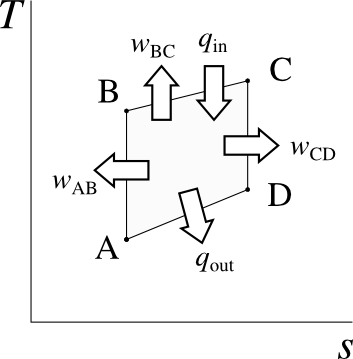
\includegraphics[width=\solutiondiagramwidth]{images/exo_sol_ts_diesel.png}
	 		\tab 2) $T_\B = \SI{1205,5}{\kelvin} = \SI{932,4}{\degreeCelsius}$ (\ref{eq_isentropique_horrible1}) ;
	 		\tab 3) $T_\C = \frac{q_\text{combustion}}{c_{p \text{(gaz)}}} + \frac{c_{p \text{(air)}}}{c_{p \text{(gaz)}}} T_\B = \SI{1984,7}{\kelvin} = \SI{1711,6}{\degreeCelsius}$ ;
	 		\tab 4) $p_\C = p_\B = \SI{158,4}{\bar}$ ;
	 		\tab 5) Avec l’\ref{eq_isentropique_horrible1}, $\frac{T_\D}{T_\C}
	 				= \left(\frac{v_\D}{v_\C}\right)^{\gamma_\text{gaz} - 1}
	 				= \left(\frac{v_\A}{v_\B} \frac{v_\B}{v_\C}\right)^{\gamma_\text{gaz} - 1}
	 				= \left[\epsilon \frac{R_\text{air}}{R_\text{gaz}} \frac{T_\B}{T_\C}\right]^{\gamma_\text{gaz} - 1}$
	 				Ainsi $T_\D = \SI{952,7}{\kelvin} = \SI{679,5}{\kelvin}$ (attention ces gaz doivent encore alimenter la turbine du turbo avant d’être éjectés dans l’atmosphère).
	 		\tab 6) $\eta_\text{moteur} = \frac{q_\net}{q_\inn} = \SI{48,06}{\percent}$ (valeur proche de la réalité car ces moteurs sont très lents et la combustion peut être faite à plus haute température encore) ;
	 		\tab 7) Voir les sections \S\ref{ch_cycle_diesel} et \S\ref{ch_cycles_pistons_reels}.
		\item [\ref{exo_cycle_turbopropulseur}]
			\tab 1) Voir \cref{fig_turbomoteur} ;
	 		\tab 2) $T_\B = \SI{6442,8}{\kelvin} = \SI{369,6}{\degreeCelsius}$ (\ref{eq_isentropique_horrible2} \& \ref{eq_puissance_compresseur}) ;
	 		\tab 3) $T_\D = \SI{976,9}{\kelvin} = \SI{703,8}{\degreeCelsius}$ (\ref{eq_isentropique_horrible2} \& \ref{eq_puissance_turbine_gaz}) ;
	 		\tab 4) $\dot W_\text{hélices} = - \dot m \ \eta_\text{transmission} \ (w_\text{turbine} + w_\text{compresseur}) = \SI{+1,517}{\mega\watt}$ (avec une efficacité thermique avant transmission de~\SI{27,6}{\percent}, valeur un peu plus faible que la réalité) ;
	 		\tab 5) Une possibilité : augmenter $\dot m_\text{air moteur}$ sans modifier les températures. Alors, $\dot m_\text{entrée~moteur~2} = \SI{5,774}{\kilogram\per\second}$ (\SI{+0,174}{\kilogram\per\second}).
		\item [\ref{exo_cycle_turboreacteur}]
			\tab 1) Voir \cref{fig_turboréacteur} ;
	 		\tab 2) $T_\B = \SI{785,2}{\kelvin}$, ainsi $T_\D = \SI{861,1}{\kelvin}$ et $T_{\D’} = \SI{783,6}{\kelvin}$ : $p_\D = \SI{3,13}{\bar}$ ;
	 		\tab 3) En négligeant $C_\D$ et avec une détente complète et réversible, $C_\E = \SI{714,3}{\metre\per\second}$ (les remarques faites en exemple \ref{exemple_tuyere} s’appliquent ici) ;
	 		\tab 4) La température en début de combustion descend à $T_3 = \SI{774,2}{\kelvin}$, la température en sortie de turbine est $T_6 = \SI{870,7}{\kelvin}$, et ainsi la pression en entrée de tuyère monte à $p_6 = \SI{4,684}{\bar}$ ;
	 		\tab 5) Gare aux tympans : $C_7= \SI{811,3}{\metre\per\second}$ (les mêmes remarques s’appliquent ici).
	 	\item [\ref{exo_cf6_generateur_intercooling}]
	 		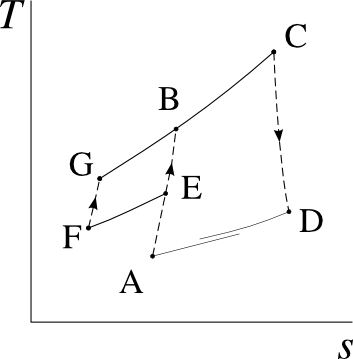
\includegraphics[width=\solutiondiagramwidth]{images/exo_sol_ts_intercooler.png}
	 		\tab 2) $\dot W_\net = \dot m \ c_{p \text{(gaz)}} \ (T_\D - T_\C) + c_{p \text{(air)}} \ (T_\B - T_\A) = \SI{-3,536}{\mega\watt}$ (environ \SI{3400}{ch}, pas trop mal pour une machine dont la première mise en route remonte à 1971… même après 15 années de service accroché sous une aile un \textsc{cf6} se vend encore plusieurs millions d’euros) ;
	 		\tab 3) $M_{w1} = \SI{38,2}{\percent}$ ;
	 		\tab 4) $\eta_1 = \SI{31,49}{\percent}$ ;
	 		\tab 6) $\dot W_{\net 2} = \SI{-3,325}{\mega\watt}$, soit une augmentation remarquable de~\SI{31}{\percent} ;
	 		\tab 7) $M_{w1} = \SI{50}{\percent}$, soit une augmentation de~\SI{+11,8}{pt} ;
	 		\tab 8) La puissance augmente de~\SI{98,8}{\kilo\joule\per\kilogram}, tandis que la consommation augmente elle de~\SI{332,6}{\kilo\joule\per\kilogram}, soit un rendement marginal de~\SI{29,7}{\percent}. L’efficacité globale diminue jusqu’à $\eta_2 = \SI{31,04}{\percent}$, soit \SI{-0,5}{pt} seulement… un compromis intéressant !
	\end{description}

